\documentclass[11pt,]{article}
\usepackage[left=1in,top=1in,right=1in,bottom=1in]{geometry}
\newcommand*{\authorfont}{\fontfamily{phv}\selectfont}
\usepackage[]{mathpazo}


  \usepackage[T1]{fontenc}
  \usepackage[utf8]{inputenc}



\usepackage{abstract}
\renewcommand{\abstractname}{}    % clear the title
\renewcommand{\absnamepos}{empty} % originally center

\renewenvironment{abstract}
 {{%
    \setlength{\leftmargin}{0mm}
    \setlength{\rightmargin}{\leftmargin}%
  }%
  \relax}
 {\endlist}

\makeatletter
\def\@maketitle{%
  \newpage
%  \null
%  \vskip 2em%
%  \begin{center}%
  \let \footnote \thanks
    {\fontsize{18}{20}\selectfont\raggedright  \setlength{\parindent}{0pt} \@title \par}%
}
%\fi
\makeatother




\setcounter{secnumdepth}{0}

\usepackage{longtable,booktabs}

\usepackage{graphicx,grffile}
\makeatletter
\def\maxwidth{\ifdim\Gin@nat@width>\linewidth\linewidth\else\Gin@nat@width\fi}
\def\maxheight{\ifdim\Gin@nat@height>\textheight\textheight\else\Gin@nat@height\fi}
\makeatother
% Scale images if necessary, so that they will not overflow the page
% margins by default, and it is still possible to overwrite the defaults
% using explicit options in \includegraphics[width, height, ...]{}
\setkeys{Gin}{width=\maxwidth,height=\maxheight,keepaspectratio}

\title{\textbf{The effect of a commercial \emph{Ascophyllum nodosum} extracts
on tomato and pepper plant productivity and their associated fungal and
bacterial communities.}  }



\author{\Large Sébastien Renaut\textsuperscript{1,2},Jacynthe
Masse\textsuperscript{1,2}, Jeffrey P. Norrie\textsuperscript{3}, Bachar
Blal\^{}\^{}3 Mohamed Hijri\textsuperscript{1,2}\vspace{0.05in} \newline\normalsize\emph{\textsuperscript{1}Département de Sciences Biologiques, Institut de
Recherche en Biologie Végétale, Université de Montréal, 4101 Sherbrooke
Est, Montreal, H1X 2B2, Quebec, Canada. \textsuperscript{2}Quebec Centre
for Biodiversity Science, Montreal, Quebec, Canada
\textsuperscript{3}Acadian Seaplant Ltd, 30 Brown Avenue, Darthmouth,
Nova Scotia, Canaad, B3B 1X8}  }


\date{}

\usepackage{titlesec}

\titleformat*{\section}{\normalsize\bfseries}
\titleformat*{\subsection}{\normalsize\itshape}
\titleformat*{\subsubsection}{\normalsize\itshape}
\titleformat*{\paragraph}{\normalsize\itshape}
\titleformat*{\subparagraph}{\normalsize\itshape}





\newtheorem{hypothesis}{Hypothesis}
\usepackage{setspace}

\makeatletter
\@ifpackageloaded{hyperref}{}{%
\ifxetex
  \PassOptionsToPackage{hyphens}{url}\usepackage[setpagesize=false, % page size defined by xetex
              unicode=false, % unicode breaks when used with xetex
              xetex]{hyperref}
\else
  \PassOptionsToPackage{hyphens}{url}\usepackage[unicode=true]{hyperref}
\fi
}

\@ifpackageloaded{color}{
    \PassOptionsToPackage{usenames,dvipsnames}{color}
}{%
    \usepackage[usenames,dvipsnames]{color}
}
\makeatother
\hypersetup{breaklinks=true,
            bookmarks=true,
            pdfauthor={Sébastien Renaut\textsuperscript{1,2},Jacynthe
Masse\textsuperscript{1,2}, Jeffrey P. Norrie\textsuperscript{3}, Bachar
Blal\^{}\^{}3 Mohamed Hijri\textsuperscript{1,2} (\textsuperscript{1}Département de Sciences Biologiques, Institut de
Recherche en Biologie Végétale, Université de Montréal, 4101 Sherbrooke
Est, Montreal, H1X 2B2, Quebec, Canada. \textsuperscript{2}Quebec Centre
for Biodiversity Science, Montreal, Quebec, Canada
\textsuperscript{3}Acadian Seaplant Ltd, 30 Brown Avenue, Darthmouth,
Nova Scotia, Canaad, B3B 1X8)},
             pdfkeywords = {Stella Maris®, 16S, ITS, soil microbial diversity, Illumina MiSeq, ANE,
Amplicon Sequence Variants, OTU},  
            pdftitle={\textbf{The effect of a commercial \emph{Ascophyllum nodosum} extracts
on tomato and pepper plant productivity and their associated fungal and
bacterial communities.}},
            colorlinks=true,
            citecolor=blue,
            urlcolor=blue,
            linkcolor=magenta,
            pdfborder={0 0 0}}
\urlstyle{same}  % don't use monospace font for urls

% set default figure placement to htbp
\makeatletter
\def\fps@figure{htbp}
\makeatother

\usepackage[left]{lineno}
\linenumbers


% add tightlist ----------
\providecommand{\tightlist}{%
\setlength{\itemsep}{0pt}\setlength{\parskip}{0pt}}

\begin{document}
	
% \pagenumbering{arabic}% resets `page` counter to 1 
%
% \maketitle

{% \usefont{T1}{pnc}{m}{n}
\setlength{\parindent}{0pt}
\thispagestyle{plain}
{\fontsize{18}{20}\selectfont\raggedright 
\maketitle  % title \par  

}

{
   \vskip 13.5pt\relax \normalsize\fontsize{11}{12} 
\textbf{\authorfont Sébastien Renaut\textsuperscript{1,2},Jacynthe
Masse\textsuperscript{1,2}, Jeffrey P. Norrie\textsuperscript{3}, Bachar
Blal\^{}\^{}3 Mohamed Hijri\textsuperscript{1,2}} \hskip 15pt \emph{\small \textsuperscript{1}Département de Sciences Biologiques, Institut de
Recherche en Biologie Végétale, Université de Montréal, 4101 Sherbrooke
Est, Montreal, H1X 2B2, Quebec, Canada. \textsuperscript{2}Quebec Centre
for Biodiversity Science, Montreal, Quebec, Canada
\textsuperscript{3}Acadian Seaplant Ltd, 30 Brown Avenue, Darthmouth,
Nova Scotia, Canaad, B3B 1X8}   

}

}








\begin{abstract}

    \hbox{\vrule height .2pt width 39.14pc}

    \vskip 8.5pt % \small 

\noindent Seaweeds have been used as a source of natural fertilizer and
biostimulants for centuries. Here, we used a commercially available
\emph{Ascophyllum nodosum} extract (ANE) in order to test its effect of
plant productivity in peppers and tomatoes. In addition, by using a
metabarcoding high throughput sequencing approach, we characteristed the
root and soil fungal and bacterial communities. We find that all
productivity measures of root, shoot and fruit biomass differed
significantly according to species, and five of those were significantly
different according to the fertilization treatment. Local
\(a\)-diversity was the highest in the bacteria-soil and fungi-soil
samples, and the lowest in the bacteria-root. In addition,
\(a\)-diversity differed according to the fertilization treatment, but
this effect were small. Species composition among sites
(\(b\)-diversity) differed according to the fertilization treatment in
all four communities measured (fungal-root, fungal-soil, bacterial-root
and bacterial-soil). Finally we identify a number of candidate taxa
(Amplicon Sequence Variants) most strongly associated with measures of
productivity. Further studies for example using inoculum of microbial
species linked to the presence of liquid seaweed extract may help to
identify a causative link between extracts, microbes and productivity.


\vskip 8.5pt \noindent \emph{Keywords}: Stella Maris®, 16S, ITS, soil microbial diversity, Illumina MiSeq, ANE,
Amplicon Sequence Variants, OTU \par

    \hbox{\vrule height .2pt width 39.14pc}



\end{abstract}


\vskip 6.5pt


\noindent \doublespacing \newpage 

\section{INTRODUCTION}\label{introduction}

Seaweeds (also known as marine macroalgae) have been used as a source of
organic matter and nutrients for centuries, especially in coastal areas
(Khan et al., 2009; Craigie, 2011). Liquid seaweed extracts, developped
in the 1950s in order to concentrate plant growth-stimulating compounds,
facilitate their usage (Milton, 1952) and today, most commercially
available extracts are made from the brown algae \emph{Ascophyllum
nodosum}, \emph{Ecklonia maxima} or \emph{Laminaria spp}. One of the
main advantages of seaweed extracts is that they are biodegradable,
non-toxic and come from a renewable resource, unlike modern chemical
fertilizers (Dhargalkar \& Pereira, 2005). Industry-funded bodies such
as the European Biostimulant Industry Coalition and the United States
Biostimulant Coalition have been working to accommodate biostimulants
into mainstream legal architecture. These organizations extoll benefits
arising from modes-of-action research, agricultural applications and
positive effects on yield and quality of many commercial species
(i.e.~fruits, vegetables, turf and ornamentals, and woody species).
Legal recognition will further allow a fluid integration of various
biostimulants, including \emph{Ascophyllum nodosum} Extracts (ANE) into
sustainable long-term crop management programs (Craigie, 2011; Jardin,
2015).\\
\hspace*{0.333em}\\
Several comprehensive reviews have described seaweed extracts and their
effect on agricultural plant productivity (Khan et al., 2009; Craigie,
2010, 2011; Battacharyya et al., 2015). The science points to
wide-ranging effects from biotic to abiotic resistance, effects on
growth and development, and ultimately, to their impact on plant
establishment, crop yield and/or quality, and shelf life. At the
physiological level, these extracts have been found to influence
hormonal changes that in turn, influence physiological processes even at
very low concentrations (Wally et al., 2013).\\
\hspace*{0.333em}\\
Starting in the 1990's, the development of high quality ANE has led to
an increase in cause-effect research, especially on plant diseases
(Jayaraj \& Ali, 2015). Noted increases in the activity of superoxide
dismutase, glutathione peroxidase and ascorbate peroxidase helped
support the argument that ANE improve plant tolerance to oxidative
stress (Ayad et al., 1997; Schmidt \& Zhang, 1997; Ayad, 1998; Allen et
al., 2001). Positive effects were also found on phytoalexin production
(Lizzi et al., 1998; Jayaraj et al., 2008; Jayaraman, Norrie \& Punja,
2010) suggesting that ANE may be involved in suppressing disease
infection through increased activity of these protective enzymes that
target oxidizing toxins naturally emitted by disease pathogens.\\
\hspace*{0.333em}\\
Improved plant stress resistance and tolerance to foliar and soil
treatments is attributed to a cascade of various physiological
reactions. ANE can impact plant-signaling mechanisms through a multitude
of plant processes and cellular modifications including
osmotic/oxidative stresses such as salinity, freezing and drought stress
(Jithesh et al., 2012). ANE can also impart drought-stress tolerance to
plants by reducing stomatal conductance and cellular electrolyte leakage
(Shotton and Martynenko, unpublished data; Spann \& Little, 2011). These
results suggest that ANE can influence cellular membrane maintenance
leading to a higher tolerance for various osmotic stresses and can
mitigate oxidative damage.\\
\hspace*{0.333em}\\
Although there is an abundance of published evidence detailing systemic
plant effects from ANE, outstanding questions remain as to the effects
of ANE on the soil rhizosphere. Various microbes, small arthropods,
nematodes, earthworms and insects thriving in the soil rhizosphere help
contribute to the aggregation of soil particles, enhance nutrient
cycling and delivery to plants, degrade toxic substances, allow better
soil water and play a role in plant disease management. An examination
of sustainable products that can positively influence microbial
interactions between plant roots and soil biota will in turn help to
further understand soil borne plant-pathogens competition dynamics. It
has been suggested that the plant immune system is composed of inherent
surveillance systems that perceive several general microbial elicitors,
which allow plants to switch from growth and development into a defense
mode (Newman et al., 2013). This may allow the plant to avoid infection
from potentially harmful microbes. The effect of ANE on the bacterial
profile suggests that ANE applications increased strawberry root and
shoot growth, berry yield and rhizosphere microbial diversity and
physiological activity (Alam et al., 2013). Similar results were found
for sandy loam soils growing carrots as Alam et al. (2014) showed a
strong relationship between carrot growth, soil microbial populations
and activity.\\
\hspace*{0.333em}\\
The recent development of culture-independent molecular techniques and
high throughput sequencing will permit to circumvent the inherent biases
of culture-based approaches by targeting the ubiquitous component of
life, its DNA. In turn, this should permit to identify a larger
proportion of the microbial diversity and lead to a better understanding
of the soil microbial response to seaweed extract. DNA barcoding
targeting the internal transcribed spacer (ITS) region of the nuclear
ribosomal repeat and the bacterial V3-V4 region of the 16S ribosomal
gene for fungi and bacteria, respectively, are now regarded as a
prerequisite procedure to comprehensively document the diversity and
ecology of microbial organisms (Toju et al., 2012; Klindworth et al.,
2013).\\
\hspace*{0.333em}\\
Here the general objective was to quantify the impact of ANE on plant
growth and test how the bacterial and fungal communities responded to
the addition of theses extracts. We also aimed to identify specific
taxon positively associated with increased in plant productivity
following addition of ANE. We hypothesized that the inclusion of liquid
seaweed extracts would improve productivity and alter significantly the
bacterial and fungal communities. We used a commercially available ANE,
Stella Maris®, developped by Acadian Plant Health (NS, Canada). Stella
Maris® is derived from the marine algae \emph{A. nodosum}, and harvested
from the nutrient-laden waters of the North Atlantic off the Eastern
Coast of Canada. We tested the effect of ANE on two commonly used plants
(tomato and pepper) using several measures of plant productivity and by
measuring soil and root bacterial and fungal diversity using High
Throughput Illumina Miseq sequencing.\\
\hspace*{0.333em}\\
\newpage  

\section{MATERIAL AND METHOD}\label{material-and-method}

\emph{Experimental design}\\
Greenhouse experiments were set up in large trays (60x30x18 cm LxWxH)
using two different crops: tomato (\emph{Solanum lycopersicum} L.) and
pepper (\emph{Capsicum annuum} L.). Tomato cultivar Totem Hybrid\#A371
was planted in November 16th 2015, while pepper cultivar Ace Hybrid\#318
was planted in December 9th 2015. Tomato and pepper seeds were purchased
from William Dam Seeds Ltd (ON, Canada). These cultivars were selected
for greenhouse production. Soil was collected from an agricultural field
under organic regime at the IRDA research station in St-Bruno (Qc,
Canada, 45\textsuperscript{o}32'59.6``N,
73\textsuperscript{o}21'08.0''W) on October 7th 2015. The soil was a
loamy sand and was collected from the 15 cm top layer. Natural soil was
mixed and put into trays, filled to 15 cm in height. Soil analysis was
done using a commercial service provided by AgriDirect (Longueuil, QC)
and soil characteristics are shown in Table 1. Eight seeds per tray were
planted and after germination, only four seedlings per tray were kept.\\
\hspace*{0.333em}\\
For each crop species, a randomized split block design (Table S1) was
used with four trays set up per block and eight blocks for each
experiment. Half of the trays were fertilized (fertilization treatment),
as described below. Half of the trays were also planted (planting
treatment) with four plants per tray, while the other trays were not
planted. This allowed a direct comparison of fungal and bacteria soil
communities with respect to fertilization and planting treatments.\\
\hspace*{0.333em}\\
Two different fertilization regimes were used according to the plant
species. For tomatoes, plants were fertilized using multipurpose organic
fertilizer (pure hen manure, 18 g per tray repeated every 4 weeks,
5-3-2) from Acti-sol (Notre-Dame-du-Bon-Conseil, QC) in addition to
Stella Maris® (3.5 ml per 1L, each tray received 250 ml, repeated every
2 weeks) for the duration of the experiment. The other half was not
fertilized. Stella Maris® is a commercial \emph{Ascophyllum nodosum}
seaweed based product and its physical and chemical analyses are shown
in Table S2 \textbf{WHERE?}. For the pepper experiment, the
fertilization regime consisted solely of Stella Maris® (3.5 ml per 1L,
each tray received 250 ml, repeated every 2 weeks) for the duration of
the experiment. The other half was not fertilized. Both experiments were
managed under organic farming practices. Thrips were controlled using
\emph{Neoseiulus cucumeris} (syn. \emph{Amblyseius cucumeris}) (1 bag
per plant), Fungus gnats were also controlled using predatory mite
\emph{Gaeolaelaps gillespiei} (1L; Natural Insect Control, ON). Plants
were treated once a week with Milstop, a Potassium Bicarbonate-based
foliar fungicide to control the powdery mildew on both crops.\\
\hspace*{0.333em}\\
\emph{Plant productivity}\\
Tomato and pepper experiments were harvested on March 29th 2016.
Measuring the following traits assessed plant productivity: fruit
number, fruit weight, shoots fresh weight and roots fresh weight. Traits
were measured on three plants chosen randomly per tray for each
fertilization-control treatment, crop (tomato/pepper) and block (eight
blocks) for a total of 96 samples. In addition, both shoots and roots
were dried in a 70 degrees drying oven, and dry weights were quantified
after 48 hours. Together, these traits are expected to represent well
the plant overall productivity.\\
\hspace*{0.333em}\\
\hspace*{0.333em}\\
\emph{Sample preparation, DNA extraction and High throughput
sequencing}\\
Soil and root samples were taken for both experiments. Soil DNA was
extracted using NucleoSpin® Soil DNA extraction kit (Macherey-Nagel,
BioLinx, ON) on 250 mg of soil, following the manufacturer's
instructions. Roots were first washed with tap water and rinsed with
sterile water. Chopped roots sub-samples (100 mg) were subjected to DNA
extraction using DNeasy Plant Mini kit (Qiagen Inc - Canada, ON),
following the manufacturer's recommendations. Amplicon sequencing
targeting bacterial 16S rRNA gene and fungal ITS was performed on both
root and soil samples.\\
\hspace*{0.333em}\\
For fungal ITS, we used the following primers with the universal CS1 and
CS2 adapters: CS1\_ITS3\_KYO2 (5'-ACA CTGA CGA CAT GGT TCT ACA GAT GAA
GAA CGY AGY RAA-3') and CS2\_ITS4\_KYO3 (5'-TAC GGT AGC AGA GAC TTG GTC
TCT BTT VCC KCT TCA CTC G-3') to produce a final amplicon size of
approximately 430bp including adapters (Toju et al., 2012).\\
\hspace*{0.333em}\\
For bacterial 16S, we used the following primers with CS1 and CS2
universal adapters: 341F (5'-CCT ACG GGN GGC WGC AG-3') and 805R (5'-GAC
TACC AGG GTA TCT AAT C-3') to produce a final amplicon size of
approximately 460 bp and targeting specifically the bacterial V3-V4
region of the 16S ribosomal gene (Klindworth et al., 2013).\\
\hspace*{0.333em}\\
DNA samples were then barcoded, pooled and sequenced (2X300bp,
paired-end) using an Illumina (San Diego, CA, USA) MiSeq sequencer
through a commercial service provided by the Genome Quebec Innovation
Centre (Montreal, QC). Sequences were demultiplexed by the sequencing
facility and further processed as described below.\\
\hspace*{0.333em}\\
\emph{Bioinformatics}\\
All bioinformatics, statistical, and graphical analyses further
described were performed in R 3.5.1 (Team, 2018) and detailed scripts
are available here
(\url{https://github.com/seb951/Acadian_Seaplants}).\\
\hspace*{0.333em}\\
We used the \texttt{R} package \texttt{dada2} (Callahan et al., 2016) to
infer \emph{Amplicon Sequence Variants} (ASVs). \texttt{Dada2} offers
accurate sample inference from amplicon data with single-nucleotide
resolution in an open source environment. Unlike the Operational
Taxonomic Unit (OTU) approach (e.g. Schloss et al., 2009; Caporaso et
al., 2010), ASV are not treated as cluster of sequences defined with an
\emph{ad hoc} sequence similarity threshold. Instead, after sequences
are quality trimmed and error-corrected, \texttt{dada2} reveals the
unique members of the sequenced community, thus allowing sequences and
abundance counts to be compared among studies (Callahan et al., 2016).\\
\hspace*{0.333em}\\
First, sequences were trimmed following strict quality thresholds
(removing primers and low quality nucleotides, see parameter details in
the accompanying \texttt{R} scripts). Following this, we applied the
error model algorithm of \texttt{dada2} which incorporates quality
information after filtering, unlike other OTU based methods. Then
dereplication, sample inference, merging of paired end reads and removal
of chimera were performed in order to obtain a sequence (ASVs) table of
abundance per sample. Taxonomy was also assigned using the Ribosomal
Database Project (RDP) Naive Bayesian Classifier algorithm from Wang
\emph{et al.} (2007). Depending on support (minimum bootstrap support of
80), we assigned taxonomy from Kingdom to species. We used the silva
database formatted for \texttt{dada2} to infer bacterial taxa (Callahan,
2018). We used the Unite (Community, 2018) fasta release (including
singletons) to infer fungal taxa after formatting it to the
\texttt{dada2} format using a custom \texttt{R} script. The pipeline was
run on a multithreaded (48 CPUs) computer infrastructure provided by
Westgrid (\url{https://www.westgrid.ca/support/systems/cedar}) and
Compute Canada (www.computecanada.ca). Note that the pipeline was run
separately for fungal-root, fungal-soil, bacteria-soil and bacteria-root
samples given the markedly different nucleotide compositions of the
sequenced amplicons, unique taxa and specific error models of each
dataset. ~\\
\hspace*{0.333em}\\
\emph{Statistical analyses - plant productivity}\\
We tested for the effect of species (tomato vs pepper), fertilization
and their interaction on six plant productivity measures (fruit number,
average fruit weight, shoots fresh weight, roots fresh weight, shoots
dry weight, roots dry weight). We used linear mixed effect models (LMM)
in the R package \texttt{nlme} (Pinheiro et al., 2017), which are more
appropriate than an Analysis of Variance (ANOVA) given the current block
design (blocks and replicates nested within a block were treated as
random variables). All six plant productivity measures were either
square root or log transformed in order to help satisfy the assumption
of normality of the residuals in the LMM statistical framework. For the
variables \emph{fruit number} and \emph{average fruit weight}, we also
used a permutation-based 2-way ANOVA (Anderson \& Legendre, 1999) given
that the residuals of the LMM were not normally distributed (results
were similarly significant).\\
\hspace*{0.333em}\\
\emph{Statistical analyses - microbial and fungal diversity}\\
Fungal-root, fungal-soil, bacterial-root and bacterial-soil ASV
diversity was measured separately. For each of these four datasets, we
removed samples that showed poor sequencing output and contained few
ASVs. In order to do this, we summed the abundance of all ASVs for each
sample (\(\sum_{i=1}^n ASV\)) and eliminated samples that had fewer that
the mean sum minus four standard deviations
(\(\overline{\sum_{i=1}^n ASV} - 4\sigma\)). In addition, we removed
ASVs from our dataset that were present in fewer than 5\% of the samples
(less than ten individuals in the soil samples or less than five in the
root samples). This was done to remove very rare ASVs unique to a block
or replicate, but not found in the majority of samples.\\
\hspace*{0.333em}\\
We then conducted community-based analyses looking at the effect of the
fertilization treatment on the ASV taxa in the tomato and pepper
experiments. To reduce the complexity of the datasets, relative
abundance of all taxa was calculated per family using the \texttt{R}
package \texttt{dplyr} (Wickham et al., 2015). Barplots were drawn using
\texttt{ggplot2} (Wickham, 2016) to visualize communities. ASV alpha
(\(a\))-diversity was calculated for each sample using the inverse
Simpson diversity index in \texttt{vegan} (Oksanen et al., 2013). The
effect of the fertilization treatment, species (and planting for soil
communities) were assessed using a linear mixed-effect (LMM) model in
the R package \texttt{nlme} (Pinheiro et al., 2017), given the
unbalanced, replicated block design. Alpha diversity was log transformed
in order to help satisfy the assumption of normality of the residuals of
the LMM statistical framework.\\
\hspace*{0.333em}\\
Using the community matrix data of ASVs abundance, we performed
PERmutational Multivariate ANalysis Of VAriance tests (PERMANOVA;
Anderson, 2001) to identify relationships between the communities
according to the experimental design. ASV abundance data was
Hellinger-transformed and significance was assessed using 10,000
permutations in \texttt{vegan} (Oksanen et al., 2013). Blocks and
replicates nested within blocks were factored as strata (blocks) in the
model.\\
\hspace*{0.333em}\\
We also performed canonical correspondence analyses (CCAs) using
Hellinger-transformed ASV abundance data in \texttt{vegan} (Oksanen et
al., 2013) to visually assess the grouping of samples, ASVs and their
association with productivity variables (\emph{species} scaling based on
ASV matrix). Data were analyzed separately for fungal-root, fungal-soil,
bacterial-root and bacterial-soil, but also according to species
(tomato/pepper), given that analyses of \(a\)-diversity showed that
tomato and pepper were markedly different. This gave a total of eight
CCAs. Data were constrained based on four productivity measures (fruit
number, average fruits weight, shoots fresh weight, roots fresh weight).
We excluded the shoot \& root dry weights as constraints to simplify the
model. In addition, these were highly correlated with the fresh weight
already included as constraints (\(r^2\)=0.98 and 0.76 for shoot
dry/fresh weights and root dry/fresh weights, respectively).\\
\hspace*{0.333em}\\
Finally, we attempted to identify candidate ASVs positively associated
with productivity. As such, we identified the ten ASVs most positively
associated with the measures of fruit number, shoots fresh weight and
roots fresh weight from each canonical correspondence analysis for a
total of 40 fungal and 40 bacterial candidate ASVs. We aligned candidate
sequences from these candidates ASVs using the Bioconductor \texttt{R}
package \texttt{decipher} (Wright, 2016) and build pairwise distances
matrices using a JC69 substitution models of DNA sequence evolution
(equal base frequencies, (Jukes \& Cantor, 1969) in \texttt{phangorn}
(Schliep, 2010). Phylogenetic trees for bacteria and fungi were plotted
using \texttt{ape} (Paradis, Claude \& Strimmer, 2004). This permitted
to identify if similar candidate ASVs were found under different
experimental conditions (soil/root, pepper/tomato), thus reinforcing
their role in productivity increase, and decreasing the false positive
rate.\\
\hspace*{0.333em}

\newpage  

\section{RESULTS}\label{results}

\emph{Soil characteristics}\\
In Table 1, we present the characteristics of the soil which was
collected at the IRDA research station in St-Bruno (Qc, Canada) and used
in the current experimental design.\\
\hspace*{0.333em}

\begin{longtable}[]{@{}lr@{}}
\caption{Soil characteristics (in ppm unless specified
otherwise)}\tabularnewline
\toprule
Soil Characteristics & Average value\tabularnewline
\midrule
\endfirsthead
\toprule
Soil Characteristics & Average value\tabularnewline
\midrule
\endhead
pH & 6.01\tabularnewline
Conductivity (mmhos/cm) & 0.68\tabularnewline
Nitrate (N) & 62.40\tabularnewline
Ammonium & 0.09\tabularnewline
Phosphorus & 0.41\tabularnewline
Potassium & 29.30\tabularnewline
Calcium & 64.40\tabularnewline
Magnesium & 13.80\tabularnewline
Chloride & 28.50\tabularnewline
Sulfate & 19.30\tabularnewline
Sodium & 17.80\tabularnewline
Zinc & 0.12\tabularnewline
Manganese & 0.06\tabularnewline
Cooper & 0.81\tabularnewline
Iron & 0.90\tabularnewline
Aluminium & 1.66\tabularnewline
\bottomrule
\end{longtable}

~\\
\hspace*{0.333em}\\
\emph{Plant productivity}\\
The effects of the fertilization treatment were tested on overall plant
growth and six measures of productivity (i.e.~fruit number, average
fruit weight, shoots fresh weight, shoots dry weight, roots fresh
weight, roots dry weight) for both tomato and peppers. Visually, both
above ground and below ground plant structure grew larger in fertilized
tomato (hen manure + ANE) and pepper plants (ANE only), in addition to
producing more fruits (see Figure 1 for some examples of the differences
between fertilized and unfertilized plants). ~\\
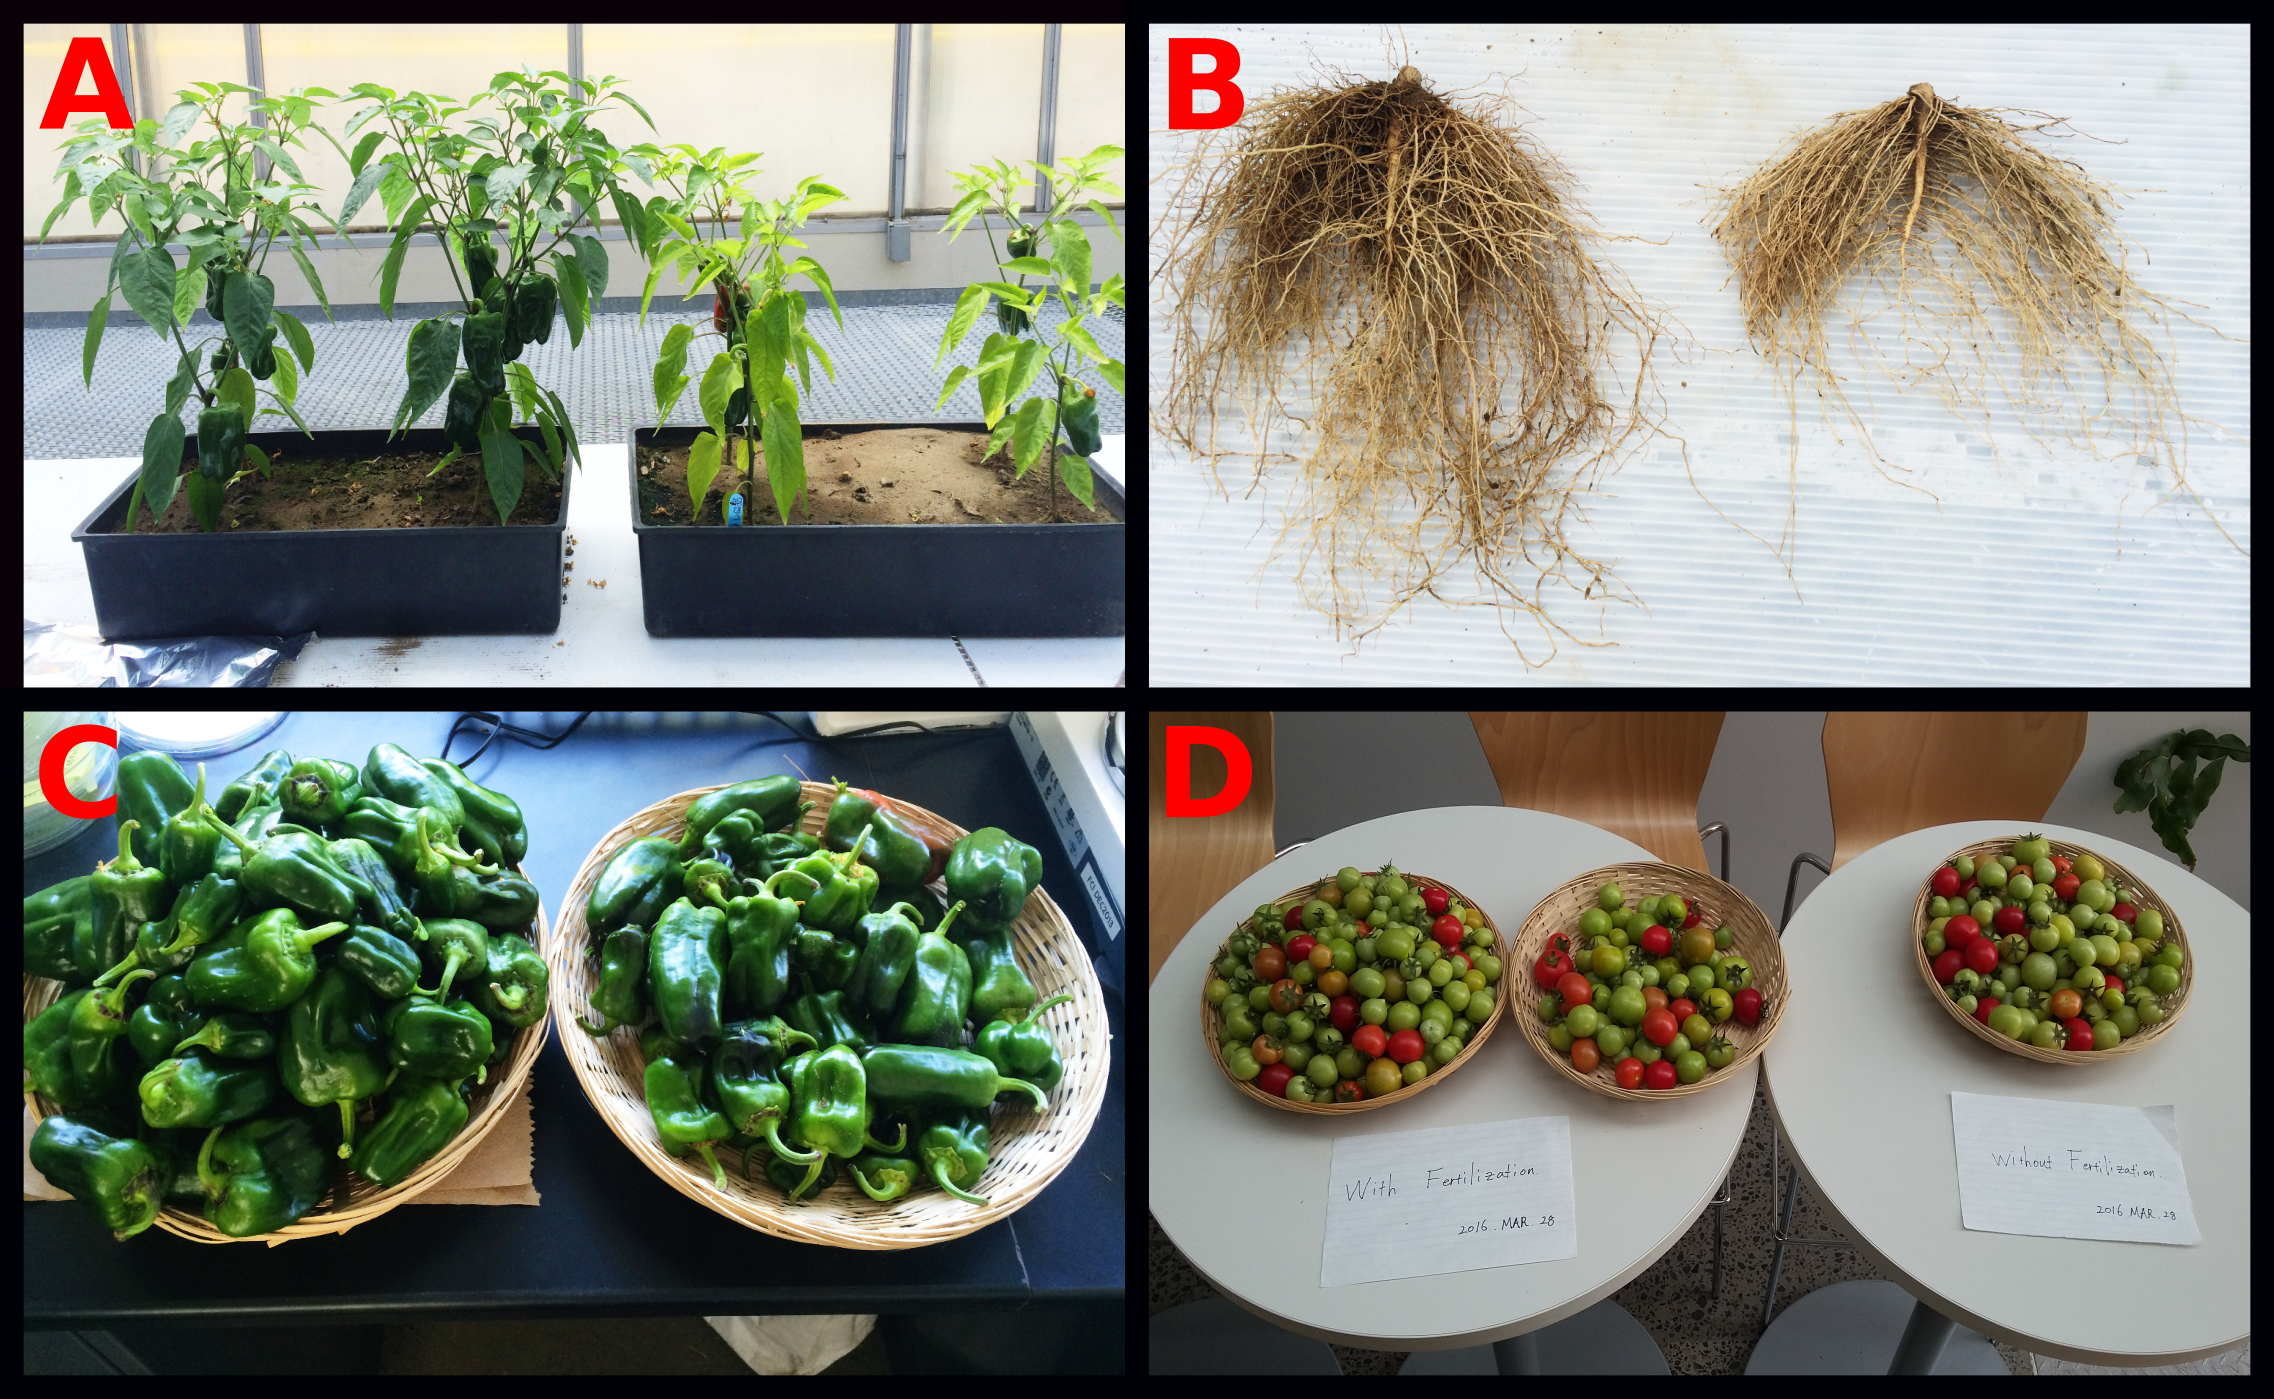
\includegraphics[width=5.20833in]{../figures/Figure_2_photos_productivity.png}\\
\textbf{Figure 1: Plant productivity. Photos were taken at the end of
the experimental treatment. In each photo, fertilized plants are on the
left. A: pepper plants, B: pepper roots, C: pepper fruits and D: tomato
fruits.}\\
\hspace*{0.333em}\\
Statistically, all six productivity measures differed significantly
according to species, and five of those were significantly different
according to the fertilization treatment (Figure 2). The fertilization
effect was stronger in the tomato plants (see fold changes in Figure 2),
likely due to the fact that these plants were fertilized with both hen
manure and ANE. The only exception was the average fruit weight that did
not differ between fertilized and control plants (LMM, \(F_{(1,69)}\) =
1.27, \emph{p}-value=0.26). However, the model did reveal a significant
interaction between treatment and plant (\(F_{(1,69)}\) = 9.6,
\emph{p}-value=0.0028). In fact, when testing only the pepper plants,
the effect of fertilization on average fruit weight was significantly
higher in the fertilized pepper plants (\(F_{(1,23)}\) = 10.84,
\emph{p}-value=0.0032).\\
\hspace*{0.333em}\\
\includegraphics[width=6.25000in]{../figures/Figure_3_productivity.pdf}\\
\textbf{Figure 2: Measures of plant productivity. \emph{a} and \emph{b}
subscripts above boxplots denote significant differences. Fold changes
between the mean of the control and fertilized plants were also noted
for significant changes (for pepper and tomato separately).}\\
\hspace*{0.333em}\\
\hspace*{0.333em}\\
\emph{Sequencing}\\
A total of 2.7 million paired-end raw reads were obtained for all
samples combined (976,000 for fungi-soil, 920,000 for fungi-root,
309,000 for bacteria-soil and 535,000 for bacteria-root, Table 2). Note
that sequencing samples were analyzed separately for fungal-soil,
fungal-root, bacteria-soil and bacteria-root conditions. On average,
47,664 paired-end reads were obtained per sample. After quality filters
were applied, including removing chimeras, and paired-end reads were
merged, an average of 19,690 sequences remained per sample. From 192
soil samples for fungi and bacteria, and 96 root samples for fungi and
bacteria sequenced, seven fungi-soil samples, 15 fungi-root samples and
one bacteria-root samples were removed because they had to few reads
based on our strict quality thresholds.\\
\hspace*{0.333em}\\
The \texttt{dada2} pipeline inferred, on average, 170 Amplicon Sequence
Variants per sample (average of 176 fungal-soil ASV, 37 fungal-root
ASVs, 269 bacterial-soil ASVs and 92 bacterial-root ASVs). Many of those
were unique to one of a few samples (total number of 6,112 fungal-soil,
845 fungal-root, 9,352 bacterial-soil and 2,023 bacterial-roots ASVs).
After quality filtering ASVs found in fewer than 10\% of the samples, we
retained 413, 106, 811 and 325 ASVs. These retained ASVs comprised 94\%,
95\%, 89\% and 98\% of all reads in the fungal-soil, fungal-root,
bacterial-soil and bacterial-root samples, respectively.\\
\hspace*{0.333em}\\
\hspace*{0.333em}

\begin{longtable}[]{@{}lrrrr@{}}
\caption{Sequencing and ASV summary}\tabularnewline
\toprule
& fungi-soil & fungi-root & bacteria-soil & bacteria-root\tabularnewline
\midrule
\endfirsthead
\toprule
& fungi-soil & fungi-root & bacteria-soil & bacteria-root\tabularnewline
\midrule
\endhead
No sequences (sum) & 976,000 & 309,000 & 920,000 &
535,000\tabularnewline
No sequences (mean) & 50,847 & 32,208 & 47,907 & 56,365\tabularnewline
No seq. filtered (mean) & 32,626 & 12,714 & 29,662 &
37,642\tabularnewline
No seq. filt. merged (mean) & 29,300 & 12,094 & 14,060 &
30,706\tabularnewline
No seq. filt. merg. no chimeras (mean) & 25,476 & 9,849 & 13,521 &
30,408\tabularnewline
No samples & 192 & 96 & 192 & 96\tabularnewline
No samples trimmed & 189 & 81 & 192 & 95\tabularnewline
No ASVs (sum) & 6,112 & 845 & 9,352 & 2,023\tabularnewline
No ASVs trimmed (sum) & 413 & 106 & 811 & 325\tabularnewline
ASV per sample (mean) & 176 & 37 & 269 & 92\tabularnewline
\bottomrule
\end{longtable}

~\\
\emph{Root, soil, microbial and bacterial diversity}\\
The entire community structure that was measurable in the soil was then
analyzed and the relative abundance of taxa (family) for the
fungal-soil, fungal-root, bacteria-soil and bacteria-root conditions was
reported (Figure 3a \& b). Fungal communities were dominated by
Nectriaceae, both in the root and soil samples. The bacterial family
Bacilaceae dominated to a lesser extent the soil communities. Bacterial
root communities were largely dominated by the Cyanobacteria phylum
(identified as \emph{chloroplast} in the silva database according to the
RDP Bayesian Classifier).\\
\hspace*{0.333em}\\
\includegraphics[width=7.29167in]{../figures/Figure4_FAMILY_barplots_fungi.pdf}\\
\textbf{Figure 3a: Barplots of the relative abundance of fungal ASVs for
fungi}\\
\hspace*{0.333em} ~\\
\includegraphics[width=7.29167in]{../figures/Figure4_FAMILY_barplots_bacteria.pdf}\\
\textbf{Figure 3b: Barplots of the relative abundance of bacterial ASVs
for bacteria}\\
\hspace*{0.333em} ~\\
\emph{Local (\(a\)-diversity)}\\
The diversity of each site (\(a\)-diversity) was calculated separately
for each sample and under each experimental condition (fungi-soil,
fungi-root, bacteria-soil and bacteria-root, Figure 4). Total
\(a\)-diversity was the highest in the bacteria-soil and fungi-soil
samples, and the lowest in the bacteria-root. Linear mixed effects
models were used to assess significance. In soil samples, fungal
diversity did not differ with respect to the fertilization
(\(F_{(1,161)}\)=0.17, \emph{p}-value=0.6853), but did so with respect
to planting (\(F_{(1,161)}\)=9.00, \emph{p}-value\textless{}0.0032) and
species (\(F_{(1,161)}\)=13.03, \emph{p}-value=0.0003) treatments. In
root samples, fungal diversity differed with respect to the
fertilization treatment (\(F_{(1,56)}\)=10.1, \emph{p}-value=0.003), and
the species tested (\(F_{(1,56)}\)=4.5, \emph{p}-value=0.04). In soil
samples, bacterial diversity differed with respect to the fertilization
(\(F_{(1,165)}\)=17.13, \emph{p}-value\textless{}0.0001), planting
(\(F_{(1,165)}\)=139.0, \emph{p}-value\textless{}0.0001) but not species
(\(F_{(1,165)}\)=1.89, \emph{p}-value=0.17) treatments. In root samples,
bacterial diversity differed with respect to the fertilization treatment
(\(F_{(1,67)}\)=17.27, \emph{p}-value=0.0001), and the species tested
(\(F_{(1,67)}\)=359.69, \emph{p}-value\textless{}0.0001). ~\\
\includegraphics[width=6.25000in]{../figures/Figure5_alpha.pdf}\\
\textbf{Figure 4: Boxplot of alpha diversity according to the treatment,
species and planting effect for fungal-root, fungal-soil, bacteria-soil
and bacteria-root. \emph{a} and \emph{b} subscripts above boxplots
denote significant differences.}\\
\hspace*{0.333em}\\
\hspace*{0.333em}\\
\emph{Differences in species composition among sites}\\
Using a PERMANOVA statistical framework, we identified that for all
conditions, communities differed with respect to the fertilization
treatment (Table 3). Soil fungal and bacterial communities differed the
most according to whether the tray was planted (greatest \% of variance
explained by factor, Table 3), while root communities differed most with
respect to the species (tomato/pepper) factor.

\begin{longtable}[]{@{}lllll@{}}
\caption{summary of the factors tested in the PERMANOVAs (\(r^2\) and
\emph{p}-values)*}\tabularnewline
\toprule
& fungi-soil & fungi-root & bacteria-soil & bacteria-root\tabularnewline
\midrule
\endfirsthead
\toprule
& fungi-soil & fungi-root & bacteria-soil & bacteria-root\tabularnewline
\midrule
\endhead
fertilization & 0.02 (2e-04) & 0.08 (1e-04) & 0.04 (1e-04) & 0.07
(1e-04)\tabularnewline
planted & 0.21 (1e-04) & NA & 0.13 (1e-04) & NA\tabularnewline
species & 0.02 (1e-04) & 0.26 (1e-04) & 0.02 (3e-04) & 0.52
(1e-04)\tabularnewline
fertilization:planted & 0.01 (0.003) & NA & 0.02 (1e-04) &
NA\tabularnewline
fertilization:species & 0.01 (0.006) & 0.04 (0.002) & 0.03 (1e-04) &
0.05 (2e-04)\tabularnewline
planted:species & 0.01 (0.09) & NA & 0.01 (0.004) & NA\tabularnewline
fertilization:planted:species & 0.01 (0.16) & NA & 0.01 (0.04) &
NA\tabularnewline
\bottomrule
\end{longtable}

*\(r^2\) (percentage of variance explained by the term in the model) and
associated \emph{p}-values in parentheses. ~\\
\hspace*{0.333em}\\
\emph{Canonical correspondence analyses and candidate ASVs}\\
Canonical correspondence analyses (CCAs) indicated how fertilized
samples clustered together according to their fungal or bacterial
communities (Figure 6). It also shows a similar association of three of
the constrain variables (productivity measures of root fresh weight,
shoots fresh weight and fruit number), while average fruit weight behave
differentially as noted previously in Figure 2 (in fact nearly
orthogonally to the other three constrains in most ordinations).\\
\hspace*{0.333em}\\
\newpage   \includegraphics{../figures/Figure6_rda.pdf}\\
\textbf{Figure 6: Canonical correspondence analyses for tomato (A-D) and
peppers (E-H) for soil-fungi, root-fungi, soil-bacteria and
root-bacteria. Samples were labeled and colored in gray (unfertilized)
or dark yellow (fertilized). Red crosses represent individual ASVs,
while red points represent the ten ASVs most closely associated with the
three productivity measures of root fresh weight, shoots fresh weight
and fruit number. Blue arrows are the four productivity measures used as
constrains in the ordinations.} ~\\
\hspace*{0.333em}\\
Next, we identified, for each ordination, the ten ASVs most closely
related to the three constrains of root fresh weight, shoots fresh
weight and fruit number. These ASVs were considered as putative
candidate sequences most positively impacted (increase presence of the
ASV) by fertilization. We further analyzed the corresponding sequences
for these eighty candidate ASVs (ten candidates * eight ordinations)in
two separate alignments (one for fungi and one for bacterial ASVs) and
their accompanying phylogenetic trees. In fungi, we identified one
cluster of ASVs taxonomically assigned to \emph{Mortierella} (soil
saprotrophs in the phylum Zygomycota) positively associated to
productivity in both tomato and pepper roots. In addition, we identified
a cluster of four different fungal ASVs in tomato soil (ASV132, ASV153)
and pepper-root (ASV19 \& AV17) closely related phylogenetically. Given
that no taxonomy was assigned to these sequences through the
\texttt{dada2} RDP bootstrap approach, we used a BLASTn (Altschul et
al., 1997) approach (against NCBI nr) to identify the most closely
related sequences. We identified this cluster of ASVs as
\emph{Rhogostoma schuessleri (BLASTn, e-value=4e-76)}, a protist in the
phylum Cercozoa, which is known to be present in the rhizo and
phyllo-sphere (Dumack et al., 2017). A number of putative plant
pathogenic fungi were also identified such as \emph{Fusarium sp.},
\emph{Microdochium colombiense} or \emph{Setophoma terrestris}. ~\\
In bacteria-roots, we identified a large number of different ASVs most
positively impacted (increase presence of the ASV) by fertilization
(Figure 6). ~\\
\hspace*{0.333em}\\
\includegraphics{../figures/Figure7_candidateASVs.pdf}\\
\textbf{Figure 6: Neighbor-Joining trees of candidates ASVs (fungi \&
roots) associated with productivity measures. The most accurate taxonomy
assigned according to the RDP bayesian classifier (form Phylum to
species) was added as tip labels.} ~\\
\hspace*{0.333em}

\newpage  

\section{DISCUSSION}\label{discussion}

In the current study, we investigated the effects of \emph{Ascophyllum
nodosum} Extracts (ANE) on root and shoot characteristics in addition to
fruit yield and bacterial and fungal communities in tomato and pepper.
Overall measures of root, shoot and fruit productivity increased for
both species following the addition of ANE. As such, our results
corrobate previous studies documenting the impact of ANE on productivity
in strawberries (Alam et al., 2013) and carrots (Alam et al., 2014).\\
\hspace*{0.333em}\\
In the tomato experimental set up, the effect of fertilization was
especially high, liley due to the fact that plants were also fertilized
with hen manure (5-3-2, 18g per tray / 2 weeks) in addition to ANE (see
Figure 2). This was not the case for the pepper plants and the increase
in productivity was solely due to the addition of ANE. The commercial
extract (Stella Maris®, Acadian Seaplants Ltd ) used contained about 1\%
nitrogen, 0.5\% phosphorus, 15\% potassium, 0.4\% calcium, 0.4\%
magnesium, 155 ppm iron, 121 ppm manganese, 5 ppm copper, 91 ppm zinc,
and 124 ppm boron. In the current experimental setup, ANE was diluted to
3.5 g / L prior to application (250ml per tray / 2 weeks). As such,
these nutrients were given at very low concentrations relative to the
crop requirements and are not expected to significantly impact growth
relative to a regular agricultural fertility program (Alam et al.,
2013). In fact, the amounts of Nitrogen and Phosphorus supplied via the
application of ANE were \textasciitilde{}100 less than from the hen
manure itself in the tomato plants. Instead, bioactive compounds such as
betaines, polyamines, cytokinins, auxins, oligosaccharides, amino acids
and vitamins have been found to have many overall beneficial
productivity effects on plant growth (Khan et al., 2009; Craigie, 2010,
2011; Battacharyya et al., 2015)\\
\hspace*{0.333em}\\
Here, one of primary goal of the study was to document how the bacterial
and fungal communities responded to the addition of ANE. We used a
metabarcoding high throughput sequencing approach targeting a DNA region
specific to all fungi (ITS) and bacteria (16S). Then, we identified
bacterial and fungal communities using a relatively novel bioinformatics
approach developed by Callahan et al. (2016). The approach, based on the
widely used programming language \texttt{R} (Team, 2018), identifies
unique, non-clustered, sequences (ASVs) that are then comparable among
studies. In the current study, most ASVs identified were rare and unique
to one or a few sample. In fact, \textasciitilde{}90\% of all ASVs were
discarded given that they were found in very few samples and were thus
not representative of a particular experimental treatment. Yet, these
ASVs comprised a small minority of all sequencing reads
(\textasciitilde{}5\% of all sequences). In addition, the current
analytical pipeline used a bayesian classifier approach to taxonomy
rather than the widely used BLAST approach, thus providing more
conservative, but more accurate taxonomic identifications (Wang et al.,
2007).\\
\hspace*{0.333em}\\
The total number of ASVs per site (\(a\)-diversity) for bacteria and
fungi differed with respect to the fertilization treatment in root
samples and the soil (only for bacteria), but these effects were small
(Figure 5). Nectriaceae, a family of fungi in the order Hypocreales and
often encountered as saprophytes on decaying organic matter comprised
most of the diversity both in the soil on root of plants (between
25-70\% of the total number of sequencing reads, Figure 4a). With
respect to soil-bacteria, communities were much more diverse and
comprised many different family (Figure 4b). Surprisingly, most
sequencing reads in the root-bacteria communities likely originate from
the plants themselves (identified as chloroplastic or mitochondrial in
origin in Figure 4b), despite the fact that the DNA primer pair used
should have primarily targeted the bacterial V3-V4 region of the 16S
ribosomal gene.\\
\hspace*{0.333em}\\
Species composition among sites (\(b\)-diversity) differed according to
the fertilization treatment in all four communities measured
(fungal-root, fungal-soil, bacterial-root and bacterial-soil). This
fertilization effect was small (2-7\% of variance explained in the
models, Table 3), but significant. Most of the variance was explained by
the planting treatment in the soil and the species (tomato/pepper) in
the roots (Table 3).\\
\hspace*{0.333em}\\
We also aimed to identify specific taxon positively associated with
increased in plant productivity following addition of ANE. Here we
discuss some of the candidates. In fungi, we identified one cluster of
ASVs taxonomically assigned to \emph{Mortierella} (soil saprotrophs in
the phylum Zygomycota) positively associated to productivity in both
tomato and pepper roots. In addition, we identified several fungal ASVs
in tomato soil and pepper-root linked to productivity. These were
assigned to \emph{Rhogostoma schuessleri (BLASTn, e-value=4e-76)}, a
protist in the phylum Cercozoa, which is known to be present in the
rhizo and phyllo-sphere (Dumack et al., 2017). A number of putative
plant pathogenic fungi were also identified such as \emph{Fusarium sp.},
\emph{Microdochium colombiense} or \emph{Setophoma terrestris}. In
bacteria-roots, we identified a large number of different ASVs most
positively impacted (increase presence of the ASV) by fertilization
(Figure 6).\\
\hspace*{0.333em}\\
DNA barcoding is now regarded as a prerequisite procedure to
comprehensively document the diversity and ecology of microbial
organisms (Toju et al., 2012; Klindworth et al., 2013). Further studies
for example using inoculum of microbial species linked to the presence
of liquid seaweed extract may help to identify a causative link between
extracts, microbes and productivity.\\
\hspace*{0.333em}\\
\hspace*{0.333em}

\section{ACKNOWLEDGMENTS}\label{acknowledgments}

We thank Mengxuan Kong for technical assistance in raising the plants
and measuring productivity and Simon Morvan for discussion about
bioinformatics analyses and seaweed extracts.

\newpage  

\section{REFERENCES}\label{references}

~

\hypertarget{refs}{}
\hypertarget{ref-alam2013effect}{}
Alam MZ., Braun G., Norrie J., Hodges DM. 2013. Effect of ascophyllum
extract application on plant growth, fruit yield and soil microbial
communities of strawberry. \emph{Canadian Journal of Plant Science}
93:23--36.

\hypertarget{ref-Alam2014}{}
Alam MZ., Braun G., Norrie J., Hodges DM. 2014. Ascophyllum extract
application can promote plant growth and root yield in carrot associated
with increased root-zone soil microbial activity. \emph{Canadian Journal
of Plant Science} 94:337--348. DOI:
\href{https://doi.org/10.4141/cjps2013-135}{10.4141/cjps2013-135}.

\hypertarget{ref-allen2001tasco}{}
Allen V., Pond K., Saker K., Fontenot J., Bagley C., Ivy R., Evans R.,
Schmidt R., Fike J., Zhang X., others. 2001. Tasco: Influence of a brown
seaweed on antioxidants in forages and livestock---A review 1.
\emph{Journal of Animal Science} 79:E21--E31.

\hypertarget{ref-altschul1997gapped}{}
Altschul SF., Madden TL., Schäffer AA., Zhang J., Zhang Z., Miller W.,
Lipman DJ. 1997. Gapped blast and psi-blast: A new generation of protein
database search programs. \emph{Nucleic acids research} 25:3389--3402.

\hypertarget{ref-anderson2001new}{}
Anderson MJ. 2001. A new method for non-parametric multivariate analysis
of variance. \emph{Austral ecology} 26:32--46.

\hypertarget{ref-anderson1999empirical}{}
Anderson MJ., Legendre P. 1999. An empirical comparison of permutation
methods for tests of partial regression coefficients in a linear model.
\emph{Journal of statistical computation and simulation} 62:271--303.

\hypertarget{ref-ayad1998effect}{}
Ayad J. 1998. The effect of seaweed extract (ascophyllum nodosum) on
antioxidant activities and drought tolerance of tall fescue (festuca
arundinacea schreb). \emph{Ph D Thesis, Texas Tech University}.

\hypertarget{ref-ayad1997effect}{}
Ayad J., Mahan J., Allen V., Brown C. 1997. Effect of seaweed extract
and the endophyte in tall fescue on superoxide dismutase, glutathione
reductase and ascorbate peroxidase under varying levels of moisture
stress. In: \emph{Proceedings}.

\hypertarget{ref-Battacharyya2015}{}
Battacharyya D., Babgohari MZ., Rathor P., Prithiviraj B. 2015. Seaweed
extracts as biostimulants in horticulture. \emph{Scientia Horticulturae}
196:39--48. DOI:
\href{https://doi.org/10.1016/j.scienta.2015.09.012}{10.1016/j.scienta.2015.09.012}.

\hypertarget{ref-silva}{}
Callahan B. 2018. Silva for dada2: Silva taxonomic training data
formatted for dada2 (silva version 132). \emph{Zenodo}. DOI:
\href{https://doi.org/10.5281/zenodo.1172783}{10.5281/zenodo.1172783}.

\hypertarget{ref-callahan2016dada2}{}
Callahan BJ., McMurdie PJ., Rosen MJ., Han AW., Johnson AJA., Holmes SP.
2016. DADA2: High-resolution sample inference from illumina amplicon
data. \emph{Nature methods} 13:581.

\hypertarget{ref-caporaso2010qiime}{}
Caporaso JG., Kuczynski J., Stombaugh J., Bittinger K., Bushman FD.,
Costello EK., Fierer N., Pena AG., Goodrich JK., Gordon JI., others.
2010. QIIME allows analysis of high-throughput community sequencing
data. \emph{Nature methods} 7:335.

\hypertarget{ref-UNITE2017}{}
Community U. 2018.UNITE general fasta release. version 01.12.2017.
\emph{Available at}
\emph{\url{https://files.plutof.ut.ee/doi/C8/E4/C8E4A8E6A7C4C00EACE3499C51E550744A259A98F8FE25993B1C7B9E7D2170B2.zip}}

\hypertarget{ref-Craigie2010}{}
Craigie JS. 2010. Seaweed extract stimuli in plant science and
agriculture. \emph{Journal of Applied Phycology} 23:371--393. DOI:
\href{https://doi.org/10.1007/s10811-010-9560-4}{10.1007/s10811-010-9560-4}.

\hypertarget{ref-craigie2011seaweed}{}
Craigie JS. 2011. Seaweed extract stimuli in plant science and
agriculture. \emph{Journal of Applied Phycology} 23:371--393.

\hypertarget{ref-dhargalkar2005seaweed}{}
Dhargalkar V., Pereira N. 2005. Seaweed: Promising plant of the
millennium.

\hypertarget{ref-dumack2017rhogostomidae}{}
Dumack K., Flues S., Hermanns K., Bonkowski M. 2017. Rhogostomidae
(cercozoa) from soils, roots and plant leaves (arabidopsis thaliana):
Description of rhogostoma epiphylla sp. nov. and r. cylindrica sp. nov.
\emph{European journal of protistology} 60:76--86.

\hypertarget{ref-duJardin2015}{}
Jardin P du. 2015. Plant biostimulants: Definition, concept, main
categories and regulation. \emph{Scientia Horticulturae} 196:3--14. DOI:
\href{https://doi.org/10.1016/j.scienta.2015.09.021}{10.1016/j.scienta.2015.09.021}.

\hypertarget{ref-Jayaraj2015sustainable}{}
Jayaraj J., Ali N. 2015. Use of seaweed extracts for disease management
of vegetable crops. In: Ganesan S, Vadivel K, Jayaraman J eds.
\emph{Sustainable crop disease management using natural products}. CAB
International, 160--183.

\hypertarget{ref-Jayaraj2008}{}
Jayaraj J., Wan A., Rahman M., Punja Z. 2008. Seaweed extract reduces
foliar fungal diseases on carrot. \emph{Crop Protection} 27:1360--1366.
DOI:
\href{https://doi.org/10.1016/j.cropro.2008.05.005}{10.1016/j.cropro.2008.05.005}.

\hypertarget{ref-Jayaraman2010}{}
Jayaraman J., Norrie J., Punja ZK. 2010. Commercial extract from the
brown seaweed ascophyllum nodosum reduces fungal diseases in greenhouse
cucumber. \emph{Journal of Applied Phycology} 23:353--361. DOI:
\href{https://doi.org/10.1007/s10811-010-9547-1}{10.1007/s10811-010-9547-1}.

\hypertarget{ref-jithesh2012analysis}{}
Jithesh MN., Wally OS., Manfield I., Critchley AT., Hiltz D.,
Prithiviraj B. 2012. Analysis of seaweed extract-induced transcriptome
leads to identification of a negative regulator of salt tolerance in
arabidopsis. \emph{HortScience} 47:704--709.

\hypertarget{ref-jukes1969evolution}{}
Jukes T., Cantor C. 1969. Evolution of protein molecules, pp. 21--132 in
mammalian protein metabolism, edited by munro hn.

\hypertarget{ref-khan2009seaweed}{}
Khan W., Rayirath UP., Subramanian S., Jithesh MN., Rayorath P., Hodges
DM., Critchley AT., Craigie JS., Norrie J., Prithiviraj B. 2009. Seaweed
extracts as biostimulants of plant growth and development. \emph{Journal
of Plant Growth Regulation} 28:386--399.

\hypertarget{ref-klindworth2013evaluation}{}
Klindworth A., Pruesse E., Schweer T., Peplies J., Quast C., Horn M.,
Glöckner FO. 2013. Evaluation of general 16S ribosomal rna gene pcr
primers for classical and next-generation sequencing-based diversity
studies. \emph{Nucleic acids research} 41:e1--e1.

\hypertarget{ref-lizzi1998seaweed}{}
Lizzi Y., Coulomb C., Polian C., Coulomb P., Coulomb P. 1998. Seaweed
and mildew: What does the future hold? \emph{Phytoma La Defense des
Vegetaux (France)}.

\hypertarget{ref-milton1952improvements}{}
Milton R. 1952. Improvements in or relating to horticultural and
agricultural fertilizers. \emph{British Patent} 664989.

\hypertarget{ref-Newman2013}{}
Newman M-A., Sundelin T., Nielsen JT., Erbs G. 2013. MAMP
(microbe-associated molecular pattern) triggered immunity in plants.
\emph{Frontiers in Plant Science} 4. DOI:
\href{https://doi.org/10.3389/fpls.2013.00139}{10.3389/fpls.2013.00139}.

\hypertarget{ref-oksanen2013package}{}
Oksanen J., Blanchet FG., Kindt R., Legendre P., Minchin PR., O'hara R.,
Simpson GL., Solymos P., Stevens MHH., Wagner H., others. 2013. Package
``vegan''. \emph{Community ecology package, version} 2.

\hypertarget{ref-paradis2004ape}{}
Paradis E., Claude J., Strimmer K. 2004. APE: Analyses of phylogenetics
and evolution in r language. \emph{Bioinformatics} 20:289--290.

\hypertarget{ref-pinheiro2017nlme}{}
Pinheiro J., Bates D., DebRoy S., Sarkar D., Team RC. 2017. Nlme: Linear
and nonlinear mixedeffects models. r package version 3.1-128. 2016.
\emph{R software}.

\hypertarget{ref-schliep2010phangorn}{}
Schliep KP. 2010. Phangorn: Phylogenetic analysis in r.
\emph{Bioinformatics} 27:592--593.

\hypertarget{ref-schloss2009introducing}{}
Schloss PD., Westcott SL., Ryabin T., Hall JR., Hartmann M., Hollister
EB., Lesniewski RA., Oakley BB., Parks DH., Robinson CJ., others. 2009.
Introducing mothur: Open-source, platform-independent,
community-supported software for describing and comparing microbial
communities. \emph{Applied and environmental microbiology}
75:7537--7541.

\hypertarget{ref-schmidt1997influence}{}
Schmidt R., Zhang X. 1997. Influence of seaweed on growth and stress
tolerance of grasses. In: \emph{Proceedings}.

\hypertarget{ref-spann2011applications}{}
Spann TM., Little HA. 2011. Applications of a commercial extract of the
brown seaweed ascophyllum nodosum increases drought tolerance in
container-grown `hamlin'sweet orange nursery trees. \emph{HortScience}
46:577--582.

\hypertarget{ref-team2018r}{}
Team RC. 2018. R: A language and environment for statistical computing.

\hypertarget{ref-toju2012high}{}
Toju H., Tanabe AS., Yamamoto S., Sato H. 2012. High-coverage its
primers for the dna-based identification of ascomycetes and
basidiomycetes in environmental samples. \emph{PloS one} 7:e40863.

\hypertarget{ref-wally2013regulation}{}
Wally OS., Critchley AT., Hiltz D., Craigie JS., Han X., Zaharia LI.,
Abrams SR., Prithiviraj B. 2013. Regulation of phytohormone biosynthesis
and accumulation in arabidopsis following treatment with commercial
extract from the marine macroalga ascophyllum nodosum. \emph{Journal of
plant growth regulation} 32:324--339.

\hypertarget{ref-wang2007naive}{}
Wang Q., Garrity GM., Tiedje JM., Cole JR. 2007. Naive bayesian
classifier for rapid assignment of rRNA sequences into the new bacterial
taxonomy. \emph{Applied and environmental microbiology} 73:5261--5267.

\hypertarget{ref-wickham2016ggplot2}{}
Wickham H. 2016. \emph{Ggplot2: Elegant graphics for data analysis}.
Springer.

\hypertarget{ref-wickham2015dplyr}{}
Wickham H., Francois R., Henry L., Müller K. 2015. Dplyr: A grammar of
data manipulation. \emph{R package version 0.4} 3.

\hypertarget{ref-wright2016using}{}
Wright ES. 2016. Using decipher v2. 0 to analyze big biological sequence
data in r. \emph{R Journal} 8.




\newpage
\singlespacing 
\end{document}
